\documentclass[a4paper, 11pt]{article}
%Paquetes%%%%%%%%%%%%%%%%%%%%%%%%%%%%%%%%%%%%%%%%%%%%%%%%%%%%%%%%%%%%%%%%%%%
\usepackage[utf8]{inputenc}
\usepackage[T1]{fontenc}
\usepackage[spanish,es-tabla]{babel}
\usepackage{everypage}
\usepackage{graphicx}
\usepackage{tikz}
\usepackage{color}
\usepackage[left=3cm, right=2.75cm, top=4.5cm, bottom=4cm]{geometry}
\usepackage{fancyhdr}
\usepackage{float}
\pagestyle{empty}
\usepackage{tikzpagenodes}
\usetikzlibrary{calc}
\usepackage{hyperref}
\usepackage{amsmath}
\usepackage{amssymb}
\usepackage{listings}
\usepackage{xcolor}
\usepackage{enumitem}
\usepackage{longtable}
\usepackage{array}
\usepackage{caption}
\captionsetup{font=small}

\definecolor{codegray}{rgb}{0.95,0.95,0.95}

\lstset{
  inputencoding=utf8,
  extendedchars=true,
  literate={á}{{\'a}}1 {é}{{\'e}}1 {í}{{\'i}}1 {ó}{{\'o}}1 {ú}{{\'u}}1
           {Á}{{\'A}}1 {É}{{\'E}}1 {Í}{{\'I}}1 {Ó}{{\'O}}1 {Ú}{{\'U}}1
           {ñ}{{\~n}}1 {Ñ}{{\~N}}1,
  backgroundcolor=\color{codegray},
  basicstyle=\ttfamily\small,
  frame=single,
  breaklines=true,
  captionpos=b,
  showstringspaces=false,
  keywordstyle=\color{blue},
  commentstyle=\color{gray},
  stringstyle=\color{red},
  numbers=left,
  numberstyle=\tiny\color{gray},
  stepnumber=1,
  numbersep=8pt,
  xleftmargin=2em,
  framexleftmargin=1.5em
}

\usepackage[user,abspage]{zref}
\renewcommand{\baselinestretch}{1.35}

\hypersetup{%
colorlinks=true, linkcolor=blue, urlcolor=blue,linkbordercolor=blue, urlbordercolor=blue, pdfborderstyle={/S/U/W 1}
}
\makeatletter
\Hy@AtBeginDocument{%
  \def\@pdfborder{0 0 1}%
  \def\@pdfborderstyle{/S/U/W 1}%
}
\makeatother
\definecolor{rojo_oscuro}{rgb}{.85,.45,.45}
\definecolor{verde_oscuro}{rgb}{0,.5,.2}
\AddEverypageHook{%
\tikz[remember picture,overlay]{%
  \ifnum\value{page}>1%
    \filldraw[fill=rojo_oscuro, thick,  draw=verde_oscuro] (1,-1.6) rectangle (16,-1.3);
    \filldraw[fill=rojo_oscuro, thick, draw=verde_oscuro] (1,-1.6-22.8) rectangle (16,-1.3-22.8);
        \node[anchor=east] at (16,-25) {\normalfont\textcolor{black}{{\footnotesize DCCO - ESPE}}};
        \node[anchor=west] at (1,-25) {\normalfont\textcolor{black}{{\footnotesize \thepage}}};
        \node at (1.8,0) {
\includegraphics[width=2.5cm]{DCCO.png}};
  \else
    \filldraw[fill=rojo_oscuro, thick, draw=verde_oscuro] (-0.3,0) rectangle (0.3,-26);
    \filldraw[fill=rojo_oscuro, thick,  draw=verde_oscuro] (1,-1.6) rectangle (16,-1.3);
    \filldraw[fill=rojo_oscuro, thick, draw=verde_oscuro] (1,-1.6-21.8) rectangle (16,-1.3-21.8);
    \node[anchor=east] at (16,-24) {\textit{{\Large Informe de historias de usuario, sprints y trazabilidad}}};
    \node[anchor=east] at (16,-25) {\textit{{\Large Ing. Jenny Ruiz}}};
    \node[anchor=east] at (16,-25.8) {\textit{{\Large Departamento de Ciencias de la Computación - ESPE}}};
    \node[anchor=east] at (16,-10) {\textbf{{\Huge Análisis y}}};
    \node[anchor=east] at (16,-11) {\textbf{{\Huge Diseño de Software}}};
    \node[anchor=east] at (16,-14.3) {\textbf{{\huge Autores}}};
    \node[anchor=east] at (16,-15.3) {\textit{{\Large Laínez Suárez Ricardo Andrés}}};
    \node[anchor=east] at (16,-16.3) {\textit{{\Large Padilla Triviño Marco Adrian}}};
    \node[anchor=east] at (16,-17.3) {\textit{{\Large Andino Martínez Nelson David}}};
    \node[anchor=east] at (16,-18.3) {\textit{{\Large NRC: 36838}}};
    \node[anchor=east] at (16,-20.6) {\textbf{{\Huge Planificación y trazabilidad}}};
    \node[anchor=east] at (16,-21.6) {\textbf{{\Huge del sistema Bocatto}}};
    \node at (4.2,0.) {
\includegraphics[width=6cm]{Logo.png}};
    \node at (14,0.) {
\includegraphics[width=2.5cm]{DCCO.png}};
  \fi}
  }
%%%%%%%%%%%%%%%%%%%%%%%%%%%%%%%%%%%%%%%%%%%%%%%%%%%%%%%%%%%%%%%%%%%%%%%%%%%
\begin{document}
\zlabel{iniciodedocumento}
\textbf{}
\newpage
\thispagestyle{empty}

\tableofcontents
\newpage

\section{Introducción}

Este informe resume cómo el Grupo 5 planificó el sistema de gestión de pedidos Bocatto y cómo se mantiene la trazabilidad de cada requisito. La planificación cubre los 8 requisitos funcionales de la ERS, con un sprint por requisito. Los sprints 1 a 4 corresponden a los casos de uso de nivel 0 trabajados en la Guía 1 y la Guía 2 (tomar pedido en mesa, realizar pedido por QR, gestionar la preparación y cobrar en caja) y están terminados. Los sprints 5 a 8 están planificados, de una semana cada uno, hasta el 15 de diciembre de 2026.

\textbf{Objetivo:} planificar los 8 requisitos y documentar la trazabilidad de los requisitos terminados (RF-02, RF-04, RF-05 y RF-06) desde la ERS hasta su historia de usuario, sus tareas en Jira, su pantalla en Confluence y su diagrama de clases generado con un prompt de ingeniería, indicando dónde se encuentra cada evidencia.

\section{Desarrollo}

\subsection{Historias de usuario (matriz MTZHU)}

Las historias de los 8 requisitos se llenaron en la plantilla de la asignatura \texttt{MTZHU\_G5\_V1.1.xlsx}. La hoja \textit{Formato descripción HU} recoge, por cada ítem, el problema, la necesidad, la solución, el usuario, las tareas, el responsable, las horas, la fecha de entrega, la prioridad, el estado, la prueba y los comentarios. La prueba indica cómo se verifica la historia y su flujo alterno, es decir, qué pasa si no se cumple. Cada historia tiene además su ficha en una hoja aparte (Figura \ref{fig:mtzhu}).

\begin{figure}[!htb]
  \centering
  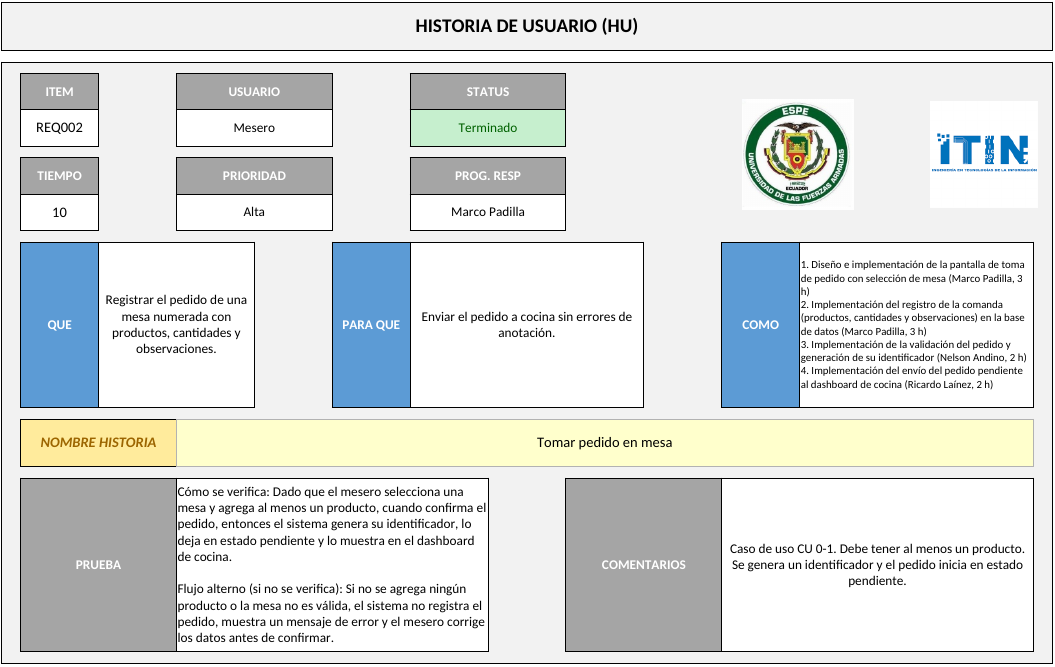
\includegraphics[width=0.56\textwidth]{mtzhu_ficha_REQ002.png}
  \caption{Ficha de la historia REQ002 en la matriz MTZHU V1.1, con la prueba y su flujo alterno.}
  \label{fig:mtzhu}
\end{figure}

\subsection{Backlog y sprints}

El backlog (\texttt{G5\_Backlog\_PlantillaV1.1.xlsx}) tiene una historia por requisito con sus subtareas \texttt{REQ00X-N}. Cada subtarea describe lo que el programador implementa, por ejemplo \textit{Diseño e implementación de la pantalla de toma de pedido con selección de mesa}. El cronograma \texttt{G5\_Cronograma\_Sprints\_V1.1.xlsx} reparte las subtareas por semana con su responsable y sus horas (Tabla \ref{tab:sprints}).

\begin{table}[H]
\centering
\footnotesize
\begin{tabular}{|l|l|l|l|l|c|l|}
\hline
\textbf{Sprint} & \textbf{Fechas} & \textbf{Requisito} & \textbf{CU} & \textbf{Encargado} & \textbf{Horas} & \textbf{Estado} \\ \hline
Sprint 1 & 8--10 nov & RF002 Tomar pedido en mesa & CU 0-1 & Marco Padilla & 10 & Terminado \\ \hline
Sprint 2 & 10--12 nov & RF004 Realizar pedido por QR & CU 0-3 & Marco Padilla & 8 & Terminado \\ \hline
Sprint 3 & 12--14 nov & RF005 Gestionar preparación & CU 0-4 & Ricardo Laínez & 8 & Terminado \\ \hline
Sprint 4 & 14--17 nov & RF006 Cobrar pedido en caja & CU 0-5 & Nelson Andino & 8 & Terminado \\ \hline
Sprint 5 & 18--24 nov & RF001 Autenticar en el sistema & CU 0-0 & Marco Padilla & 12 & Planificado \\ \hline
Sprint 6 & 25 nov--1 dic & RF003 Tomar pedido telefónico & CU 0-2 & Ricardo Laínez & 11 & Planificado \\ \hline
Sprint 7 & 2--8 dic & RF008 Administrar configuración & CU 0-7 & Ricardo Laínez & 13 & Planificado \\ \hline
Sprint 8 & 9--15 dic & RF007 Consultar estado de pedido & CU 0-6 & Nelson Andino & 9 & Planificado \\ \hline
\end{tabular}
\caption{Sprints, requisitos y encargados. Las subtareas suman 79 h: 30 h de Marco Padilla, 26 h de Ricardo Laínez y 23 h de Nelson Andino.}
\label{tab:sprints}
\end{table}

\subsection{Jira}

En el proyecto Scrum \textbf{36838\_G5} cada sprint es una épica que agrupa su historia. Cada historia lleva el requisito en el nombre y, en una descripción corta, la historia de usuario, el caso de uso, la prioridad, el criterio de aceptación, el flujo alterno y la trazabilidad. Sus subtareas tienen responsable y horas. Los sprints 1 a 4 están cerrados con sus historias finalizadas y los sprints 5 a 8 están creados como sprints futuros.

\begin{figure}[!htb]
  \centering
  \begin{minipage}{0.49\textwidth}
    \centering
    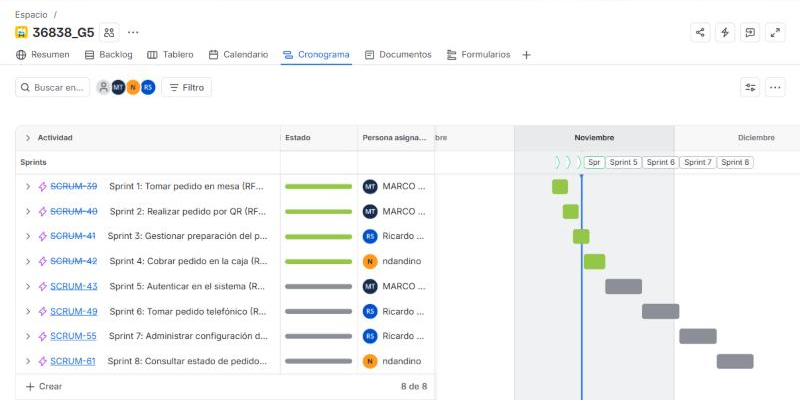
\includegraphics[width=\textwidth,height=3.6cm,keepaspectratio]{jira_cronograma_8RF.png}
  \end{minipage}\hfill
  \begin{minipage}{0.49\textwidth}
    \centering
    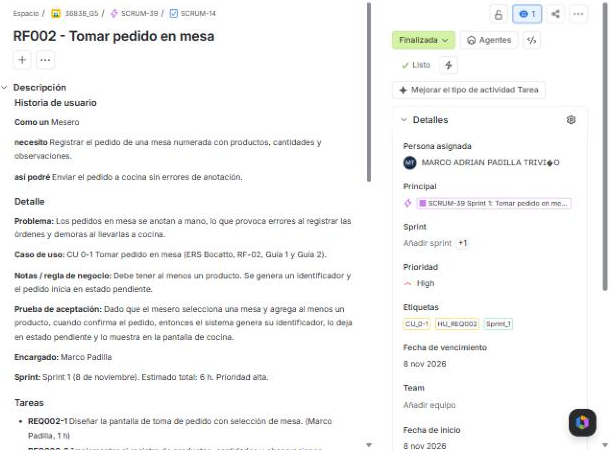
\includegraphics[width=\textwidth,height=3.6cm,keepaspectratio]{jira_historia_RF002.png}
  \end{minipage}
  \caption{Cronograma de Jira con las 8 épicas (izquierda) e historia SCRUM-14 con su descripción (derecha).}
  \label{fig:jira}
\end{figure}

\subsection{Confluence}

En el espacio 36838\_G5, la página \textit{Maquetado del sistema Bocatto por requisito} tiene una subpágina por requisito y otra con el modelo de datos. Cada subpágina muestra la historia de usuario, el sprint y el encargado, el enlace a Jira, la trazabilidad, la prueba de aceptación, el flujo alterno, el mockup de la pantalla, el diagrama de clases, los datos que usa y las reglas de negocio (Figura \ref{fig:conf}, izquierda).



\subsection{Trazabilidad con prompt y diagrama de clases}

Para cada requisito se redactó un requisito atómico y se usó un modelo de lenguaje con un prompt de ingeniería para generar el código PlantUML de su diagrama de clases. El prompt original se incorporó dentro del código como comentario de metadatos con las etiquetas \texttt{/' ... '/}. Así, el modelo queda ligado al requisito, al caso de uso, a la historia y a la tarea de Jira. El fragmento siguiente corresponde a REQ002 y su diagrama está en la Figura \ref{fig:conf}, a la derecha.

\begin{lstlisting}[basicstyle=\ttfamily\scriptsize]
' REQ002_TomarPedidoMesa.txt
@startuml
/'
METADATOS DE TRAZABILIDAD
Requisito: REQ002 (RF-02) | Caso de uso: CU 0-1 | Jira: SCRUM-14 (Sprint 1)
Prompt: Actúa como un Analista de Software y Diseñador UML. Con base en el siguiente requisito atómico, genera el código PlantUML de un Diagrama de Clases que modele la ontología básica de esta funcionalidad (frontera, controlador, entidades y persistencia desacoplada)...
Requisito Atómico: "El sistema Bocatto deberá permitir al Mesero registrar el pedido de una mesa numerada con sus productos, cantidades y observaciones..."
'/
\end{lstlisting}

\begin{figure}[!htb]
  \centering
  \begin{minipage}{0.52\textwidth}
    \centering
    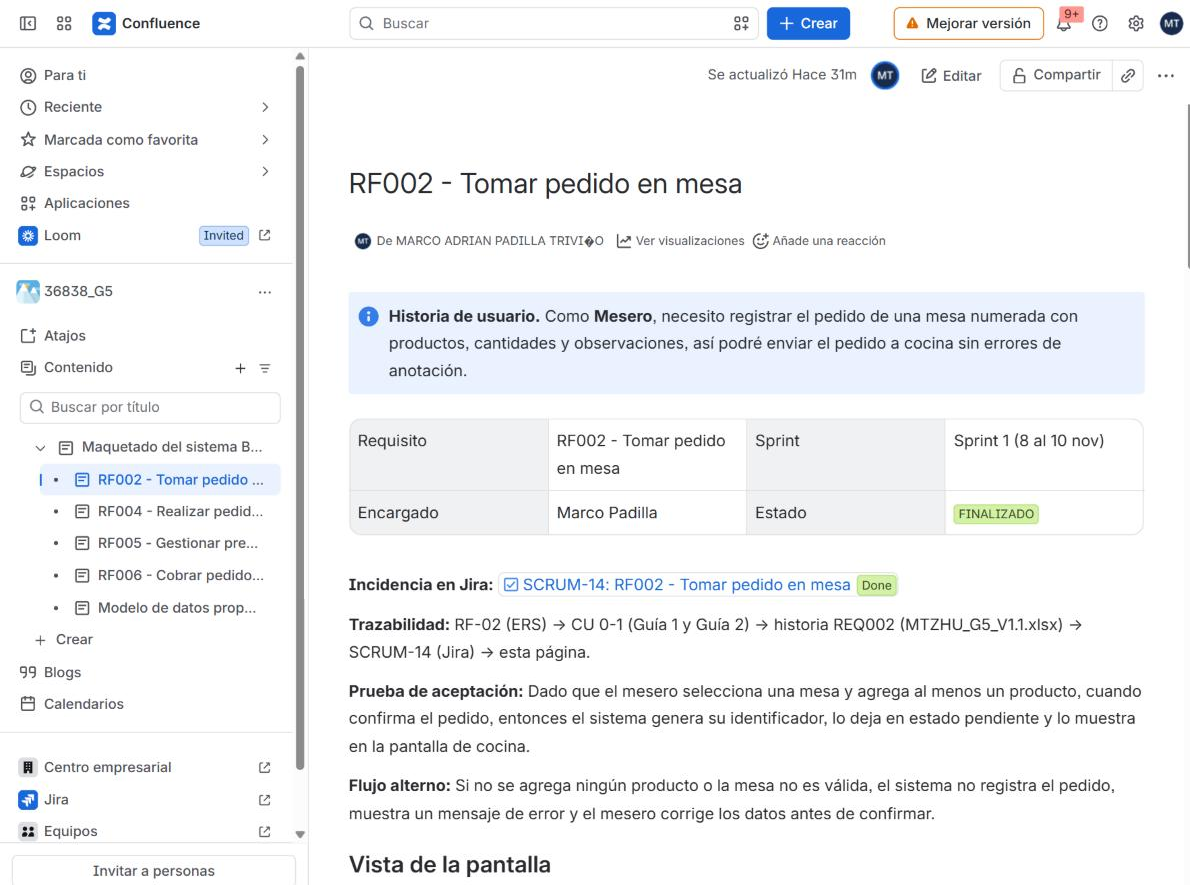
\includegraphics[width=\textwidth,height=3.4cm,keepaspectratio]{confluence_rf002.png}
  \end{minipage}\hfill
  \begin{minipage}{0.44\textwidth}
    \centering
    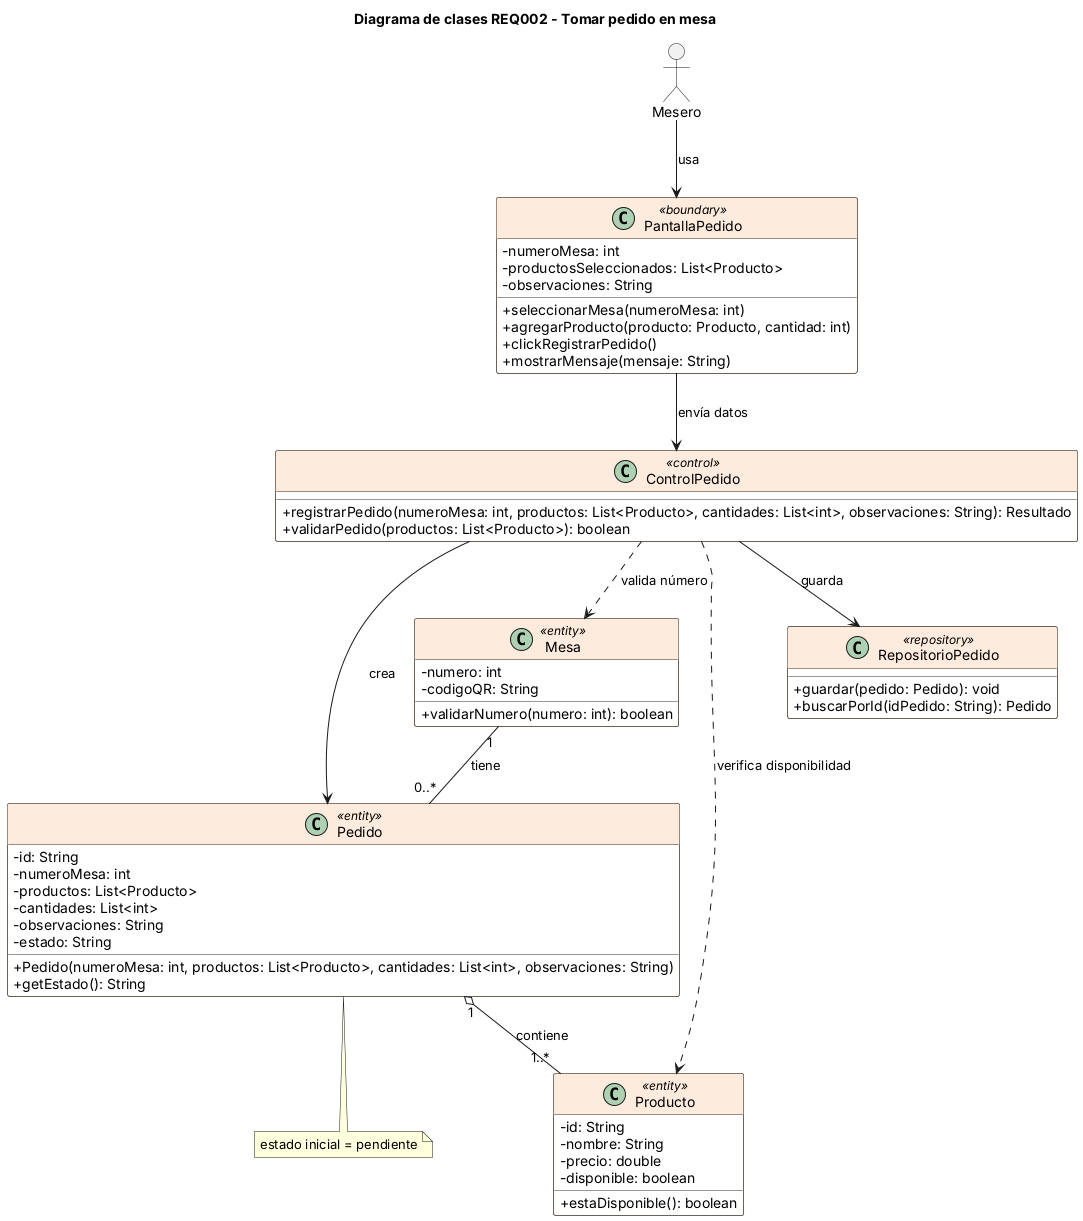
\includegraphics[height=3.5cm]{REQ002_TomarPedidoMesa.png}
  \end{minipage}
  \caption{Página de Confluence de RF002 con su trazabilidad (izquierda) y diagrama de clases de REQ002 generado a partir del prompt (derecha).}
  \label{fig:conf}
\end{figure}

La ficha de trazabilidad de cada requisito está en el README de \texttt{1.8 Archivos de Respaldo}.

\subsection{Dónde está cada evidencia}

El repositorio se organizó en la carpeta \texttt{PROYECTO}, con \texttt{1. ELICITACION}, \texttt{2. DISEÑOS} y \texttt{3. CODIGO}. En Notion, la sección \textit{SPRINTS - JIRA} del espacio P.A.R.A. tiene la tabla de los 8 sprints con un enlace por sprint, y la pestaña \textit{Archivos} guarda cada documento con su archivo original y su enlace a GitHub (Figura \ref{fig:donde}).

\begin{figure}[!htb]
  \centering
  \begin{minipage}{0.52\textwidth}
    \centering
    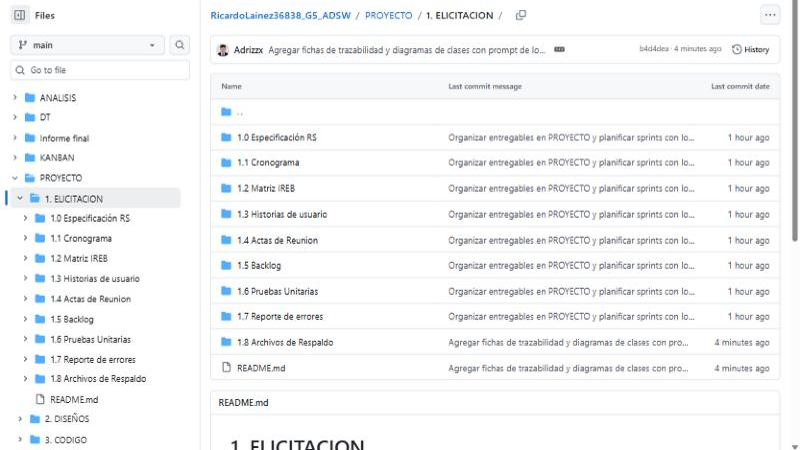
\includegraphics[width=\textwidth,height=2.6cm,keepaspectratio]{github_proyecto.png}
  \end{minipage}\hfill
  \begin{minipage}{0.40\textwidth}
    \centering
    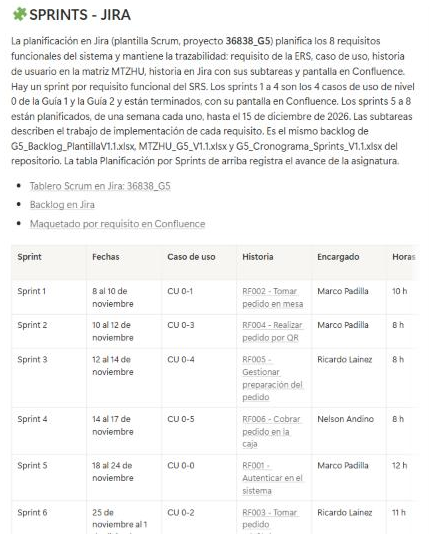
\includegraphics[width=\textwidth,height=2.6cm,keepaspectratio]{notion_sprints.png}
  \end{minipage}
  \caption{Carpeta de elicitación en GitHub (izquierda) y sección SPRINTS - JIRA en Notion (derecha).}
  \label{fig:donde}
\end{figure}

{\footnotesize
\begin{longtable}{|p{3.4cm}|p{10.8cm}|}
\caption{Ubicación de cada evidencia.}\label{tab:links}\\
\hline
\textbf{Evidencia} & \textbf{Ubicación} \\ \hline
\endfirsthead
\hline
\textbf{Evidencia} & \textbf{Ubicación} \\ \hline
\endhead
Historias de usuario & \href{https://github.com/Ricardo-lainez/RicardoLainez36838_G5_ADSW/tree/main/PROYECTO/1.\%20ELICITACION/1.3\%20Historias\%20de\%20usuario}{PROYECTO/1. ELICITACION/1.3 Historias de usuario} \\ \hline
Backlog y cronograma & \href{https://github.com/Ricardo-lainez/RicardoLainez36838_G5_ADSW/tree/main/PROYECTO/1.\%20ELICITACION/1.5\%20Backlog}{1.5 Backlog} y \href{https://github.com/Ricardo-lainez/RicardoLainez36838_G5_ADSW/tree/main/PROYECTO/1.\%20ELICITACION/1.1\%20Cronograma}{1.1 Cronograma} \\ \hline
Fichas de trazabilidad & \href{https://github.com/Ricardo-lainez/RicardoLainez36838_G5_ADSW/tree/main/PROYECTO/1.\%20ELICITACION/1.8\%20Archivos\%20de\%20Respaldo}{PROYECTO/1. ELICITACION/1.8 Archivos de Respaldo} \\ \hline
Diagramas de clases & \href{https://github.com/Ricardo-lainez/RicardoLainez36838_G5_ADSW/tree/main/PROYECTO/2.\%20DISE\%C3\%91OS/2.5\%20Diagramas\%20de\%20clases\%20por\%20requisito}{PROYECTO/2. DISEÑOS/2.5 Diagramas de clases por requisito} \\ \hline
Guías, mockups y modelo & \href{https://github.com/Ricardo-lainez/RicardoLainez36838_G5_ADSW/tree/main/PROYECTO/2.\%20DISE\%C3\%91OS}{PROYECTO/2. DISEÑOS} (2.1, 2.2 y 2.3 Mockups) \\ \hline
Jira (tablero) & \href{https://36838-g5.atlassian.net/jira/software/projects/SCRUM/boards/1}{36838-g5.atlassian.net/jira/software/projects/SCRUM/boards/1} \\ \hline
Confluence & \url{https://36838-g5.atlassian.net/wiki/spaces/3/pages/327682} \\ \hline
Notion (P.A.R.A.) & \url{https://www.notion.so/3f3cd8194c458048b3adf5c09e2195b6} \\ \hline
NotebookLM & \href{https://notebook.google.com/notebook/eca2758b-8588-4cd0-880c-3fe946384210}{Cuaderno del proyecto (19 fuentes)} \\ \hline
Gem Tutor Bocatto & \url{https://gemini.google.com/gem/d9eeb390f7c5?usp=sharing} \\ \hline
\end{longtable}
}

\section{Conclusiones}

Los 4 requisitos terminados se siguen sin saltos desde la ERS hasta su diagrama de clases, y los otros 4 ya tienen historia, subtareas y sprint hasta el 15 de diciembre. El prompt dentro del código PlantUML deja registrado cómo se obtuvo cada modelo.

\end{document}
